\documentclass[Softwaredesign/Softwaredesign_main.tex]{subfiles}
\begin{document}
GUI er implementeret i form af en UI QT design fil,  en C++  klasse samt en qrc ressource fil. UI filen står for selve udsenet af GUI'en; hvor at C++ klassen står for opførslen af GUI'en. qrc ressource filen er en fil som bruges til at tilgå de forskellige billeder som bruges i GUI'en. 

UI filen har en liste over QObjekter som bliver implementeret Display delen af RPiapp'en, de kan ses på figur \ref{fig:Qobj_list}. Disse objekter er logisk implementeret af QT creator i en form for HTML, kaldt QML. Men da QT Creator har en "drag and drop" menu, er det muligt at undgå at skrive dette manuelt.  
\begin{figure}[H]
    \centering
    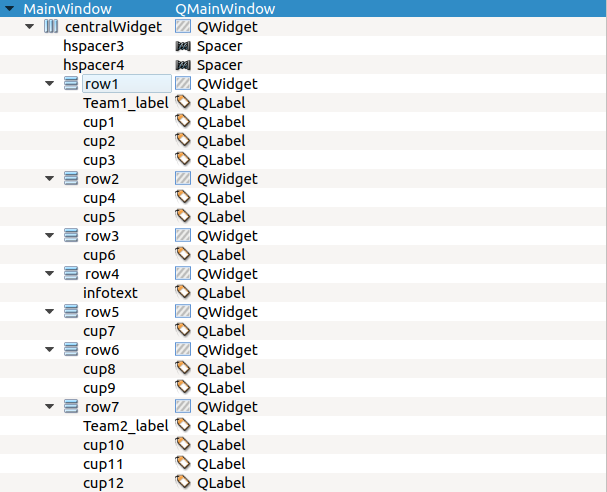
\includegraphics[scale=0.7]{Softwaredesign/GUI/Pictures/Liste_af_Qobjekter.png}
    \caption{Liste af QObjekter som bruges i Display delen af RPiapp'en.}
    \label{fig:Qobj_list}
\end{figure}


\begin{figure}[H]
    \centering
    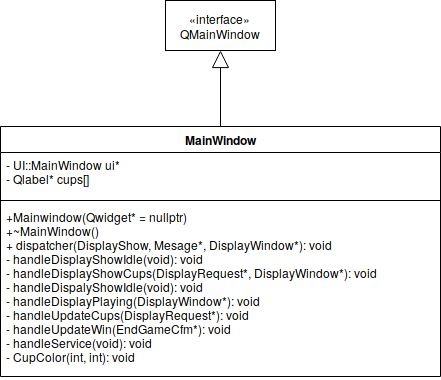
\includegraphics{Softwaredesign/GUI/Pictures/Mainwindow_klasse.png}
    \caption{Klassediagram}
    \label{fig:Mainwindow_klasse_dia}
\end{figure}

Alle funktioner som kan ses på figur \ref{fig:Mainwindow_klasse_dia}, kan ses implementeret:

\textbf{Constructor}
\begin{verbatim}
MainWindow::MainWindow(QWidget *parent) :
    QMainWindow(parent),
    ui(new Ui::MainWindow)
{
    ui->setupUi(this);

    cups[0] = ui->cup1;
    cups[1] = ui->cup2;
    cups[2] = ui->cup3;
    cups[3] = ui->cup4;
    cups[4] = ui->cup5;
    cups[5] = ui->cup6;

    cups[6] = ui->cup7;
    cups[7] = ui->cup8;
    cups[8] = ui->cup9;
    cups[9] = ui->cup10;
    cups[10] = ui->cup11;
    cups[11] = ui->cup12;
}
\end{verbatim}

\textbf{Destructor}
\begin{verbatim}
MainWindow::~MainWindow()
{
    delete ui;
}
\end{verbatim}


\textbf{Dispatcher}
I dispatcher tages tre argumenter: id, msg, og arg. "id"  bruges som det som trigger switchen, alt efter hvilken type besked som sendes.  msg pointeren indeholder forskelligt data, alt efter hvilken type besked der sendes. Hvis det f.eks. er en EndGameCfm message, så indeholde hvilken side der tabte. DisplayWindow pointeren skal bruges når det skal haves adgang direkte til bruger data, f.eks. hvis man skal finde hvilke kopper hold 1 har. 
\begin{verbatim}
void MainWindow::dispatcher(DisplayShow id, Message * msg, DisplayWindow* arg)
{
    switch (id)
    {
    case _IDLE:
        this->handleDisplayShowIdle();
    break;
    case _INFO:
        this->handleDisplayShowInfo();
    break;
    case _GAME_STATUS:
        this->handleDisplayPlaying(arg);
    break;
    case ENDGAME:
        this->handleUpdateWin(static_cast<EndGameCfm *>(msg));
    break;
    case _SERVICE:
          this->handleService();
    break;
    case _CUPS_UPDATED:
         this->handleUpdateCups(static_cast<DisplayRequest *>(msg), arg);
    break;
    case _PLACE_CUPS:
        this->handleDisplayShowPlaceCups();
    break;
    default:
    break;
    }}
\end{verbatim}


\textbf{HandleDisplayShowIdle}
ShowIdle funktionen er rimelig simpelt,  alle labels bliver sat til at være tomme,  og stylesheet'et bliver sat til at være IDLE\_SHEET.
\begin{verbatim}
void MainWindow::handleDisplayShowIdle()
{
    ui->infotext->setText("");
    ui->Team1_label->setText("";
    ui->Team1_label->setText("");
    this->setStyleSheet(IDLE_SHEET);
}
\end{verbatim}


\textbf{HandleDisplayShowPlaceCusp}
ShowPlaceCups sætter info teksten til at fortælle bruger(ne) , at de skal placere kopperne.
\begin{verbatim}
void MainWindow::handleDisplayShowPlaceCups()
{
    ui->infotext->setText("Place DEM CUPS!");
}
\end{verbatim}


\textbf{HandleDisplayShowInfo}
DisplayShowInfo sætter info teksten til at fortælle bruger(ne), at de skal indtaste info på hjemmesiden.
\begin{verbatim}
void MainWindow::handleDisplayShowInfo()
{
    ui->infotext->setText("Enter info at THE website");
}
\end{verbatim}


\textbf{HandleDisplayPlaying}
DisplayPlaying sætter et spil igang. Den tager en DisplayWindow poniter for at få adgang til: holdnavne og brugernavne, derefter sættes de til at være de udledte navne. Derefter sættes stylesheet'et til at vise gameboarded.  Alle kopperne sættes til at være grønne, da alle kopperne er på plads.  Tilsidst sættes info teksten til at være tom,  da alt der var krævet af brugerne nu er gjort.  
\begin{verbatim}
void MainWindow::handleDisplayPlaying(DisplayWindow* arg)
{
    const std::string team1 = arg->getTeam1()->getTeam() + "\n" + arg->getTeam1()->getUser1() + "\n" + arg->getTeam1()->getUser2();
    const std::string team2 = arg->getTeam2()->getTeam() + "\n" + arg->getTeam2()->getUser1() + "\n" + arg->getTeam2()->getUser2();

    ui->Team1_label->setText(QString::fromStdString(team1));
    ui->Team2_label->setText(QString::fromStdString(team2));

    this->setStyleSheet(GAMEBOARD_SHEET);

    int i = 0;
    for(i=0;i>11;i++)
    {
        cups[i]->setStyleSheet(GREENCUP_SHEET);
    }
    ui->infotext->setText("");
}
\end{verbatim}

\textbf{HandleUpdateCups}
UpdateCups tager en Displayequest pointer og en DisplayWinow pointer. Displayrequest pointeren fortæller funktionen hvilket hold som skal have deres kopper opdateret. Følgende bruges DisplayWindow pointeren til at tilgå information omkring hvilke kopper er aktive for en given bruger. 
\begin{verbatim}
void MainWindow::handleUpdateCups(DisplayRequest* arg, DisplayWindow* pointer)
{

    std::cout << "UPDATE CUPS HANDLER WAS USED" << std::endl;
    if(arg->playerside_==1)
    {
        bitset<6> kopper = pointer->getTeam1()->getCups();
        int i= 0;
        for(i=0;i==5;i++)
        {
            if(kopper[i] == true)
            {
                cups[i]->setStyleSheet(GREENCUP_SHEET);
            }
            else if(kopper[i] == false)
            {
                cups[i]->setStyleSheet(REDCUP_SHEET);
            }
        }
    }

    if(arg->playerside_==2)
    {
        bitset<6> kopper = pointer->getTeam2()->getCups();
        int i= 0;
        for(i=0;i==5;i++)
        {
            if(kopper[i] == true)
            {
                cups[i]->setStyleSheet(GREENCUP_SHEET);
            }
            else if(kopper[i] == false)
            {
                cups[i]->setStyleSheet(REDCUP_SHEET);
            }}}}
\end{verbatim}


\textbf{HandleUpdateWin}
UpdateWin tager en EndGameCfm poniter. Beskeden indeholder hvilken side som har tabt spillet.  Den information bruges til at bestemme hvilket "victory sheet" der skal vises, og sheet'et bliver sat som givet. Desuden bare for en sikkerheds skyld så tømmes alle tekstbokse.
\begin{verbatim}
void MainWindow::handleUpdateWin(EndGameCfm * msg)
{
    ui->infotext->setText("");
    ui->Team1_label->setText("");
    ui->Team2_label->setText("");

     if(msg->looserPlayerside_ == 1)
    {
        this->setStyleSheet(VICTORY2_SHEET);
    }
    else if(msg->looserPlayerside_ == 2)
    {
       this->setStyleSheet(VICTORY1_SHEET);
    }
}
\end{verbatim}


\textbf{HandleService}
Service funktionen tømmer alle tekstbokse,  i tilfælde af der skulle være noget tekst som ikke skal være der.  Derefter sættes sheet'et til at vise service skærmen. 
\begin{verbatim}
void MainWindow::handleService()
{
    ui->infotext->setText("");
    ui->Team1_label->setText("");
    ui->Team2_label->setText("");

    this->setStyleSheet(SERVICE_SHEET);
}
\end{verbatim}




\end{document}